\documentclass[12pt,letterpaper]{article}
\usepackage[utf8]{inputenc}	% Para caracteres en español
\usepackage{amsmath,amsthm,amsfonts,amssymb,amscd}
\usepackage[table]{xcolor} 
\usepackage[margin=3cm]{geometry}
\usepackage{ragged2e}
\usepackage{graphicx}
\usepackage{hyperref}
\usepackage{amssymb}
\usepackage{subfigure}
\newlength{\tabcont}
\setlength{\parindent}{0.0in}
\setlength{\parskip}{0.05in}

\begin{document}
	
	\begin{table}[]
		\centering
		\label{my-label}
		\begin{tabular}{llll}
			\textbf{Nomes:}&Luís Felipe de Melo Costa Silva &   \textbf{Nº USP:} & 9297961 \\
			& Nícolas Nogueira Lopes da Silva &         & 9277541 \\
		\end{tabular}
	\end{table}
	
	\begin{center}
		\huge \bf
		Exercício-Programa II de MAC0210 \\
	\end{center}
	
	\section{Parte 0 - Laboratório}
	
	Nesta parte do problema tivemos que fazer a implementação das funções que servirão para o estudo da interpolação de polinômios aplicados a imagens. As decisões de projeto e detalhes da implementação estão descritos abaixo. 
	
	Vale lembrar que as funções trabalham com imagens com três canais de cores. Portanto, quando nos referirmos a um ponto de uma matriz, na verdade estaremos nos referindo a um vetor de três coordenadas, onde cada coordenada representa uma cor (no caso, vermelho, verde e azul, respectivamente). As matrizes que usamos têm três dimensões.
	
	\subsection{compress.m}
	
	Esse arquivo contém apenas uma função, a \texttt{compress}, com o seguinte protótipo:
	
	\begin{center}
		\texttt{function compress (originalImg, k)}
	\end{center}
	
	Ela recebe um arquivo de imagem no formato \textit{png} e devolve, em um outro arquivo \textit{png}, a imagem comprimida com a taxa $k$.
	
	A leitura da imagem recebida é armazenada em uma matriz grande. Comprimimos retirando todas as linhas e colunas $i$ tal que $i\%(k+1)=1$, onde $\%$ representa a operação de resto.
	
	A compressão é feita sequencialmente, analisando a matriz grande por pontos. Quando encontramos um par (linha, coluna) em que as duas satisfazem o requisito, o atribuímos à matriz pequena. O ponto $(x, y)$ da matriz grande é colocado no seguinte ponto da matriz pequena:  $(\left \lfloor{\frac{x}{k+1}+1}\right \rfloor, \left \lfloor{\frac{y}{k+1}+1}\right \rfloor)$.
	
	Feito isso, a matriz pequena é escrita numa imagem \textit{png}.

	\subsection{calculateError.m}
	
	O arquivo possui apenas uma função, a \texttt{calculateError}, que tem o protótipo:
	
	\begin{center}
		\texttt{function calculateError(originalImg, decompressedImg)}
	\end{center}
	
	Essa função calcula o erro relativo entre duas imagens (aqui, usamos para a imagem comprimida e uma imagem descomprimida), usando as fórmulas fornecidas no enunciado.
	
	\clearpage
	
	Primeiramente, lemos as imagens e armazenamos em matrizes, então, fazemos a conta. Não há muito segredo aqui. O único detalhe da implementação é que usamos a função \texttt{norm} do Octave para calcular a norma euclidiana.
	
	\subsection{decompress.m}
	
	Esse é o function file mais importante dos três enviados. Ele faz a descompressão de uma imagem usando algum método de interpolação e nos devolve o arquivo com a imagem descomprimida. Ele possui as seguintes funções, com os protótipos:
	
	\begin{center}
		\texttt{function decompress (compressedImg, method, k, h)}
	\end{center}
	
	A função \texttt{decompress} recebe uma imagem em \textit{png} e a descomprime em uma razão $k$, utilizando o método bilinear ou o método bicúbico.
	
	Ela lê a imagem e a armazena em uma matriz. A descompressão será feita inserindo $k$ linhas e colunas entre as linhas e colunas da matriz. Calculamos o tamanho da $p$ da imagem descomprimida usando a fórmula $p = n+(n-1)\cdot k$, onde $n$ é o tamanho da matriz da imagem pequena.
	
	Dependendo do método escolhido pelo usuário, ela chama a função que desenvolverá o método da interpolação, que devolverá uma matriz com os pontos interpolados.
	
	Feito isso, essa matriz é escrita em um arquivo \textit{png}.

	\begin{center}
		\texttt{function B = bilinear (A, k, h, p)}
	\end{center}
	
	Esse representa um dos métodos de interpolação descrito no enunciado, o método Bilinear por partes.
	
	Para começar, chamamos a função \texttt{expande}, que nos devolve uma matriz com o tamanho que precisamos (mais detalhes abaixo).
	
	Com essa matriz definimos quadrados de lado $k+2$ e, então, armazenamos os vértices do quadrado. Usamos \texttt{X = inv(A)*B} para resolver o sistema linear do método da interpolação (no enunciado está na forma B = AX). Com a matriz X dos valores da solução, fazemos a interpolação para cada cor de todos os pontos dentro de cada quadrado definido, usando a fórmula dada:
	
	\begin{center}
		$f(x, y) \approx p_{ij} (x, y) = a_0 + a_1(x - x_i ) + a_2 (y - y_j ) + a_3 (x - x_i )(y - y_j)$
	\end{center}
	
	No entanto, fizemos pequenas adaptações para a implementação funcionar:
	
	\begin{center}
		\texttt{f = X(1) + X(2).*x + X(3).*y + X(4).*x.*y;}, onde:
	\end{center}
	
	\begin{itemize}
		\item \texttt{f} é o resultado do polinômio interpolador.
		\item \texttt{X(i)} é o correspondente a $a_{i-1}$, proveniente da solução do sistema linear.
		\item \texttt{x} e \texttt{y} são as coordenadas do ponto no quadrado, definidos assim:
		\begin{itemize}
			\item \texttt{x = ((m-i)/(k+1))*h;}, onde $m$ é a real coordenada do ponto na matriz, $i$ é o início do quadrado na matriz grande, $k$ é a taxa de descompressão e $h$ é referente ao lado do quadrado, definido no enunciado.
			\item \texttt{y = ((n-j)/(k+1))*h;}, onde $n$ é a real coordenada do ponto na matriz, $j$ é o início do quadrado na matriz grande, e o resto é análogo.
		\end{itemize}
		\item Isso faz com que os pontos usados para a interpolação vão de 0 a $h$.
	\end{itemize}
	
	O cálculo é feito para todos os pontos que não são os vértices do quadrado. 
	
	Em nosso método, consideramos $(x_0, y_0)$ como $(1, 1)$ da matriz e $(x_{p-1}, y_{p-1})$ como $(p, p)$ da matriz.
	 
	\begin{center}
		\texttt{function B = bicubico (A, k, h, p)}
	\end{center}

	Essa função representa o outro método de interpolação descrito no enunciado, o método Bicubico.

	Da mesma forma que no outro método, chamamos a função \texttt{expande} que devolve uma matriz com o tamanho necessário (mais detalhes abaixo).

	Para o cálculo das derivadas parciais existem 3 funções: \texttt{derivax}, \texttt{derivay} e \texttt{derivaxy} que já verificam as condições para as derivadas na borda. Uma observação a se realizar é que consideramos que nos casos em que aparecem pontos que extrapolam a grade fizemos os cálculos utilizando a diferença unilateral com o ponto da borda e seu adjacente.

	Para cada quadrado $Q_{ij}$ descrito no enunciado calculamos a matriz com os 16 coeficientes de $p_{ij}$. Calculamos os valores das cores de cada pixel da imagem com a fórmula do polinômio interpolador para cada quadrado $Q_{ij}$ do enunciado.

	\begin{center}
		\texttt{function B = expande (A, k, p)}
	\end{center}
	
	Essa função faz algo parecido com o oposto do descrito em \textbf{compress.m}
	
	Recebe uma matriz quadrada $A$ de tamanho $p$ e coloca $k$ linhas e colunas de zeros entre suas linhas e colunas, atribuindo tudo isso em uma matriz $B$. 
	
	Vamos andando ponto a ponto, e caso esse ponto tenha o par (linha, coluna) = $(i, j)$ tal que ambos os números cumpram o requisito $x\%(k+1)=1$, onde $\%$ representa a operação de resto, o correspondente $(\frac{i-1}{k+1}+1, \frac{j-1}{k+1}+1)$ da matriz $A$ é atribuído na matriz $B$.
	
	\section{Parte 1 - Zoológico}
	
	Para os experimentos do zoológico, utilizamos as seguintes imagens: 
	
	\begin{figure}[h]
		\subfigure[Figura 1\label{surreal1}]{
		
\includegraphics[width=6.5cm,height=6.5cm]{zoo1.png}}
		\subfigure[Figura 1 em preto e branco.\label{surreal2}]{
		
\includegraphics[width=6.5cm,height=6.5cm]{zoo1a.png}}
	\end{figure}
	
	\begin{figure}[h]
		\subfigure[Figura 2\label{surreal11}]{
			
\includegraphics[width=6.5cm,height=6.5cm]{zoo3.png}}
		\subfigure[Figura 3\label{surreal21}]{
			
\includegraphics[width=6.5cm,height=6.5cm]{zoo2.png}}
	\end{figure}
	
	\begin{itemize}
		\item Figura 1: gerada através da função
		$f(x,y) = (sen(x), \frac{sen(y)+sen(x)}{2}, sen(x)$, descrita no enunciado (281 por 281 pixels);
		\item Figura 2: gerada através da função $f(x,y) = (cos(x), 2\cdot cos(y), x^2)$ (281 por 281 pixels);
		\item Figura 3: gerada por $f(x,y) = (tan(x) - tan(y), tan(y)- y, tan(x))$ (505 por 505 pixels).
	\end{itemize}
	
	\clearpage
	
	\subsection{Usando o método Bilinear}
	
	Usando o método Bilinear, descomprimimos as imagens, e obtivemos as seguintes respostas para as perguntas do enunciado:
	
	\textbf{1.} Funciona bem para imagens preto e branco?\\
	Sim, pois comparando com uma imagem colorida, o erro não foi muito diferente.\\
	
	\textbf{2.} Funciona bem para imagens coloridas?\\
	Funciona. As imagens ficam visualmente parecidas e o erro fica pequeno (a maioria na ordem de $10^{-2}$)\\
	
	\textbf{3.} Funciona bem para todas as funções de classe $C^2$?\\
	Sim, como exemplificado pelas figuras 1 e 2.\\
	
	\textbf{4.} E para funções que não são de classe $C^2$? \\
	Também funciona, como na figura 3.\\
	
	\textbf{5.} Como o valor de h muda a interpolação? \\
	O valor de h não parece interferir tanto na interpolação, pois, como exibido abaixo pelas figuras (g) e (h), que foram descomprimidas com h diferente ($h = 5$ e $h = 7$), o erro ficou muito próximo.\\
	
	\textbf{6.} Como se comporta o erro?\\
	Os erros ficaram bem pequenos, como exibido abaixo. Foi interessante ver que mudando a cor de uma imagem seu erro muda, e que quanto menor o $h$ usado para compressão e descompressão, menor o erro. \\
	
	\textbf{7.} Considerando uma imagem de tamanho $p^2$, comprimida com $k = 7$ e descomprimida com $k = 7$ e com $k = 1$ três vezes, quais são as conclusões?\\
	As imagens ficam pareceidas visualmente, porém o erro é menor (como mostram as imagens (h) e (i)).
.
	Abaixo, seguem as imagens acima descomprimidas.
	
	\begin{figure}[h]
		\subfigure[1 descomprimida com h = 4 e k = 3, err = 0.76841\label{surreal12}]{
		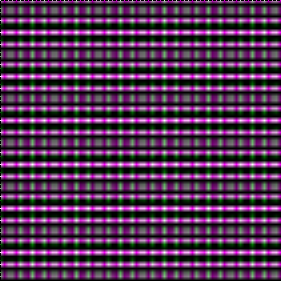
\includegraphics[width=5cm,height=5cm]{zdec1.png}}
		\subfigure[1 descomprimida com h = 4 e k = 3, err = 0.77409 \label{surreal22}]{
		
\includegraphics[width=5cm,height=5cm]{zdec1a.png}}
	\end{figure}
	
	\clearpage
	
	\begin{figure}[h]
		\subfigure[2 descomprimida com h = 5 e k = 7, err = 1.0884\label{surreal13}]{
			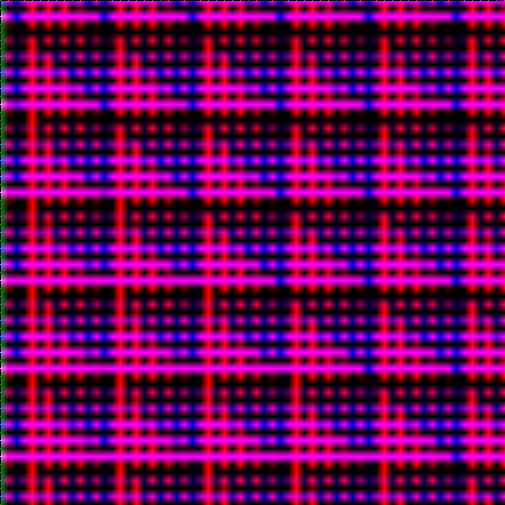
\includegraphics[width=5cm,height=5cm]{zdec2.png}}
		\subfigure[2 descomprimida com h = 7 e k = 7, err = 1.0884\label{surreal23}]{
			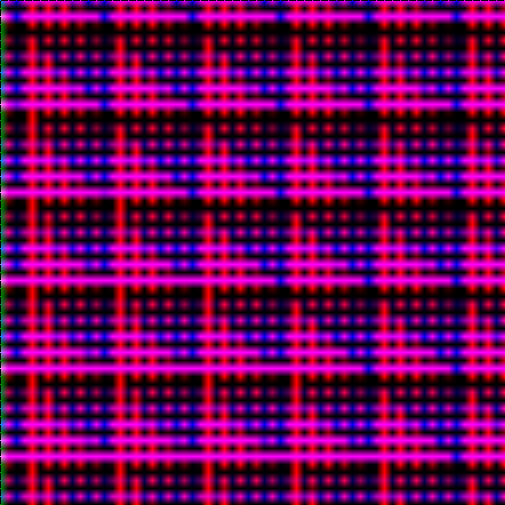
\includegraphics[width=5cm,height=5cm]{zdec2a.png}}
	\end{figure}
	
	\begin{figure}[h]
		\subfigure[2 descomprimida com h = 2 e k = 1 três vezes, err = 0.09700\label{surreal28}]{
		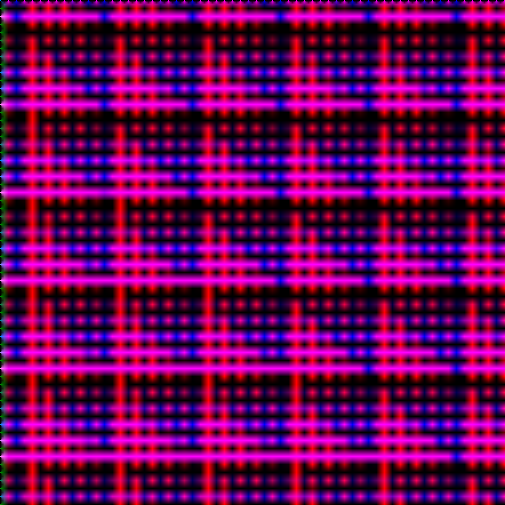
\includegraphics[width=5cm,height=5cm]{zdec2b.png}}
		\subfigure[3 descomprimida com h = 2 e k = 4, err = 0.66150\label{surreal18}]{
		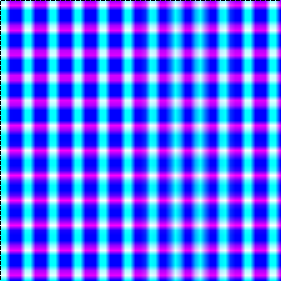
\includegraphics[width=5cm,height=5cm]{zdec3.png}}
	\end{figure}
	
	Obs: As imagens foram comprimidas e descomprimidas com o mesmo k, para manter o tamanho e o cálculo do erro ser facilitado.
	
	\subsection{Usando o método Bicúbico}

	Usando o método Bicúbico, descomprimimos as imagens, e obtivemos as seguintes respostas para as perguntas do enunciado:
	
	\textbf{1.} Funciona bem para imagens preto e branco?\\
	\\
	
	\textbf{2.} Funciona bem para imagens coloridas?\\
	\\
	
	\textbf{3.} Funciona bem para todas as funções de classe $C^2$?\\
	\\
	
	\textbf{4.} E para funções que não são de classe $C^2$? \\
	\\
	
	\textbf{5.} Como o valor de h muda a interpolação? \\
	\\
	
	\textbf{6.} Como se comporta o erro?\\
	\\
	
	\textbf{7.} Considerando uma imagem de tamanho $p^2$, comprimida com $k = 7$ e descomprimida com $k = 7$ e com $k = 1$ três vezes, quais são as conclusões?\\
	
	Abaixo, seguem as imagens acima descomprimidas.
	
	\begin{figure}[h]
		\subfigure[1 descomprimida com h = 4 e k = 3, err = 0.85446\label{surreal12}]{
		
\includegraphics[width=5cm,height=5cm]{zbicdec1.png}}
		\subfigure[1 descomprimida com h = 4 e k = 3, err = 0.82142 \label{surreal22}]{
		
\includegraphics[width=5cm,height=5cm]{zbicdec1a.png}}
	\end{figure}
	
	\clearpage
	
	\begin{figure}[h]
		\subfigure[2 descomprimida com h = 5 e k = 7, err = 1.0321\label{surreal13}]{
			
\includegraphics[width=5cm,height=5cm]{zbicdec2a.png}}
		\subfigure[2 descomprimida com h = 7 e k = 7, err = 1.0322\label{surreal23}]{
			
\includegraphics[width=5cm,height=5cm]{zbicdec2b.png}}
	\end{figure}
	
	\begin{figure}[h]
		\subfigure[2 descomprimida com h = 2 e k = 1 três vezes, err = 1.0208\label{surreal28}]{
		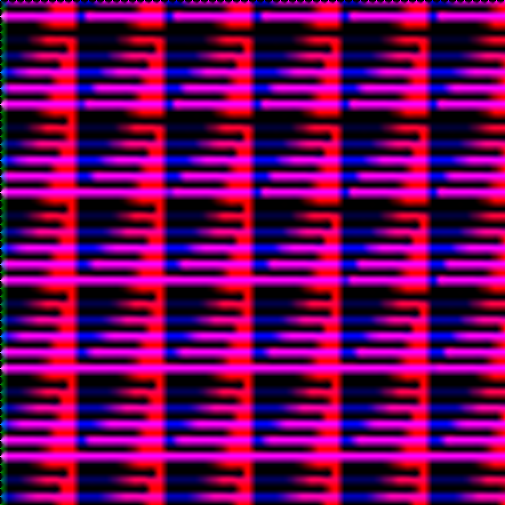
\includegraphics[width=5cm,height=5cm]{zbicdec2c.png}}
		\subfigure[3 descomprimida com h = 2 e k = 4, err = 0.88062\label{surreal18}]{
		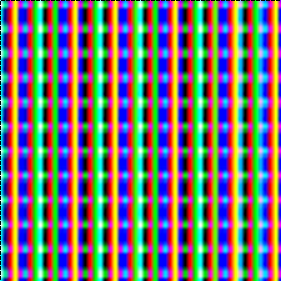
\includegraphics[width=5cm,height=5cm]{zbicdec3.png}}
	\end{figure}
	
	Obs: As imagens foram comprimidas e descomprimidas com o mesmo k, para manter o tamanho e o cálculo do erro ser facilitado.
	
	\section{Parte 2 - Selva}
	
	Para a selva, utilizamos as seguintes imagens:
	\clearpage
	
	\begin{figure}[h]
		\subfigure[Figura 4\label{surreal14}]{
		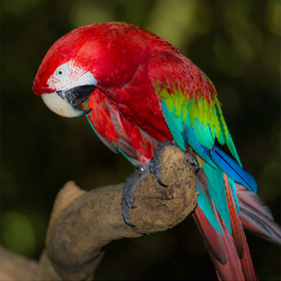
\includegraphics[width=3cm,height=3cm]{1.png}}
		\subfigure[Figura 5.\label{surreal24}]{
		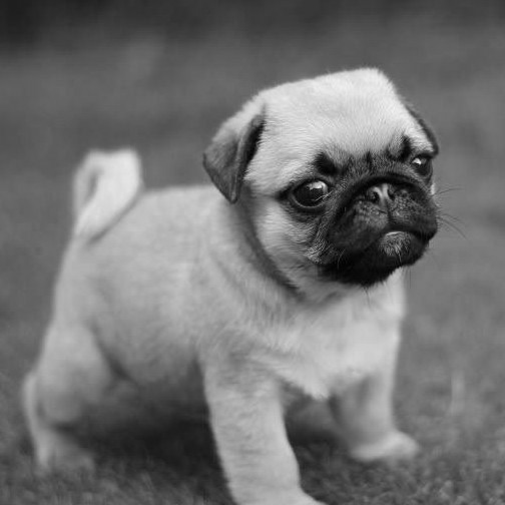
\includegraphics[width=3cm,height=3cm]{2.png}}
		\subfigure[Figura 6\label{surreal34}]{
		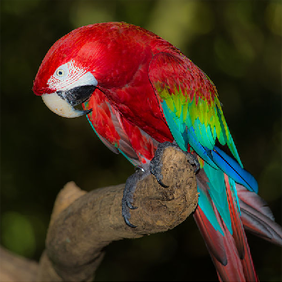
\includegraphics[width=3cm,height=3cm]{3.png}}
		\subfigure[Figura 7\label{surreal44}]{
		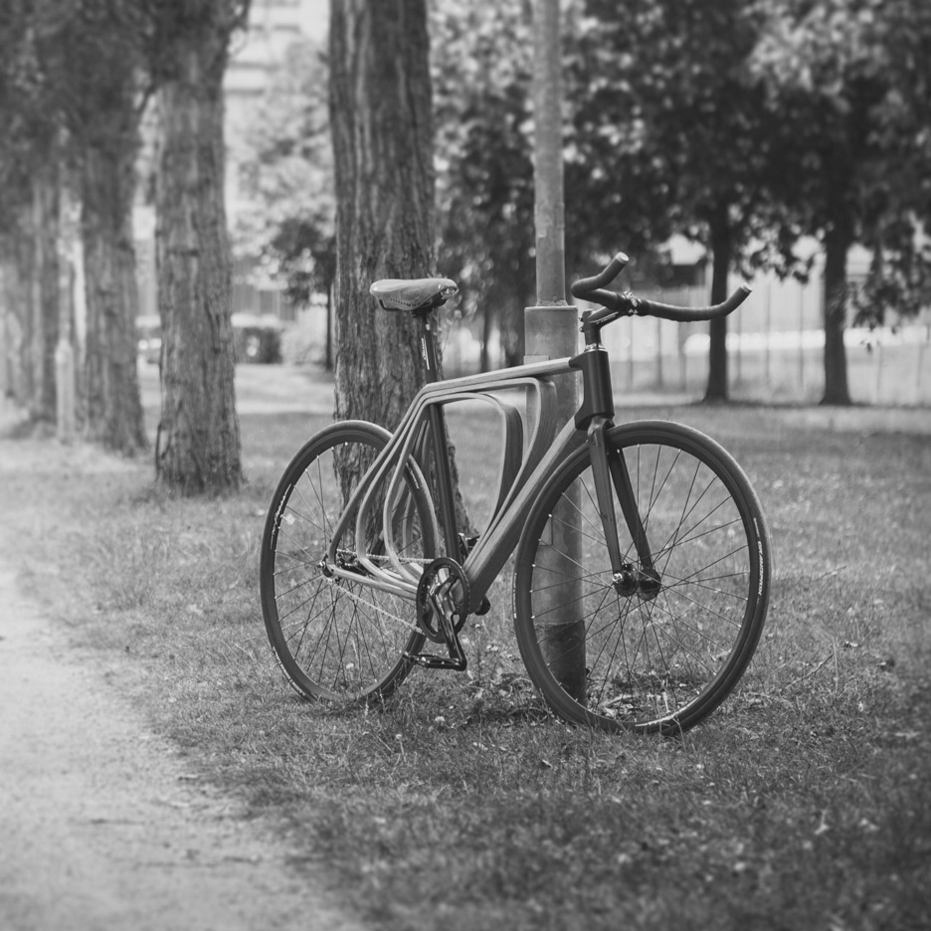
\includegraphics[width=3cm,height=3cm]{4.png}}
	\end{figure}
	
	\begin{itemize}
		\item Figura 4: Arara (colorida) (281 por 281 pixels);
		\item Figura 5: Cachorro (preto e branco) (505 por 505 pixels);
		\item Figura 6: Maçãs (colorida) (505 por 505 pixels);
		\item Figura 7: Bicicleta (preto e branco) (931 por 931 pixels).
	\end{itemize}
	
	\subsection{Usando o método Bilinear}
	
	Usando o método Bilinear, descomprimimos as imagens, e obtivemos as seguintes respostas para as perguntas do enunciado:
	
	\textbf{1.} Funciona bem para imagens preto e branco?\\
	Sim, pois comparando com uma imagem colorida de mesmo tamanho, o erro fica diferente, mas pequeno.\\
	
	\textbf{2.} Funciona bem para imagens coloridas?\\
	Também unciona. As imagens ficam visualmente parecidas e o erro fica pequeno (a maioria na ordem de $10^{-2}$)\\
	
	\textbf{3.} Como o valor de h muda a interpolação? \\
	Em imagens reais, o valor de h não parece interferir tanto na interpolação, pois, como exibido abaixo pelas figuras (q) e (r), que foram descomprimidas com h diferente ($h = 3$ e $h = 5$), o erro ficou muito próximom, mas parece diminuir quando $h$ aumenta.\\
	
	\textbf{4.} Como se comporta o erro?\\
	Os erros ficaram bem pequenos, como exibido abaixo. Foi interessante ver que mudando a cor de uma imagem seu erro muda, e que quanto menor o $h$ usado para compressão e descompressão, menor o erro, como mostrado pelas imagens (o) e (p). \\
	
	\textbf{5.} Considerando uma imagem de tamanho $p^2$, comprimida com $k = 7$ e descomprimida com $k = 7$ e com $k = 1$ três vezes, quais são as conclusões?\\
	As imagens ficam pareceidas visualmente, porém o erro é maior (como mostram as imagens (s) e (t)).
	
	Seguem as descomprimidas:
	
	\begin{figure}[h]
		\subfigure[4 descomprimida com h = 4 e k = 3, err = 0.057654\label{surreal15}]{
		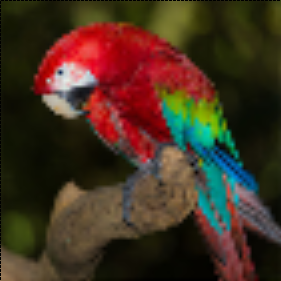
\includegraphics[width=5cm,height=5cm]{decompressed1.png}}
		\subfigure[4 descomprimida com h = 4 e k = 4, err = 0.065963 \label{surreal25}]{
		
\includegraphics[width=5cm,height=5cm]{decompressed1a.png}}
	\end{figure}
	
	\begin{figure}[h]
		\subfigure[5 descomprimida com h = 3 e k = 7, err = 0.033480\label{surreal16}]{
		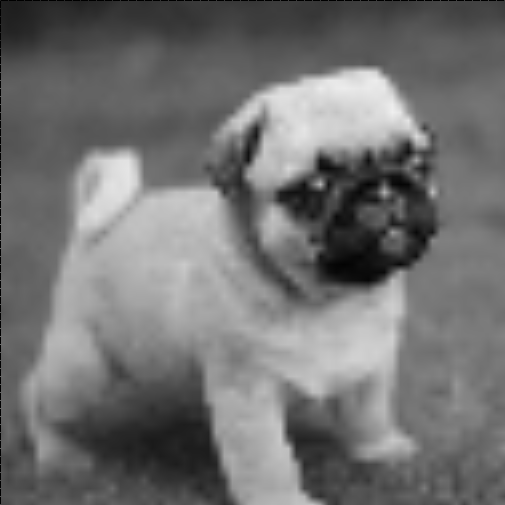
\includegraphics[width=5cm,height=5cm]{decompressed2.png}}
		\subfigure[5 descomprimida com h = 5 e k = 7, err = 0.033479\label{surreal26}]{
			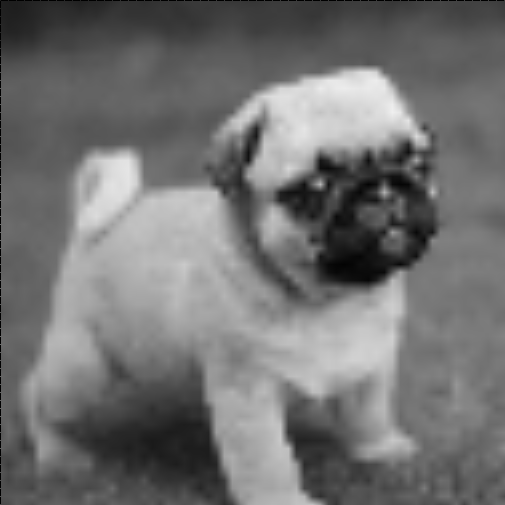
\includegraphics[width=5cm,height=5cm]{decompressed2a.png}}
	\end{figure}
	
	\begin{figure}[h]
		\subfigure[6 descomprimida com h = 2 e k = 7, err = 0.080604\label{surreal17}]{
		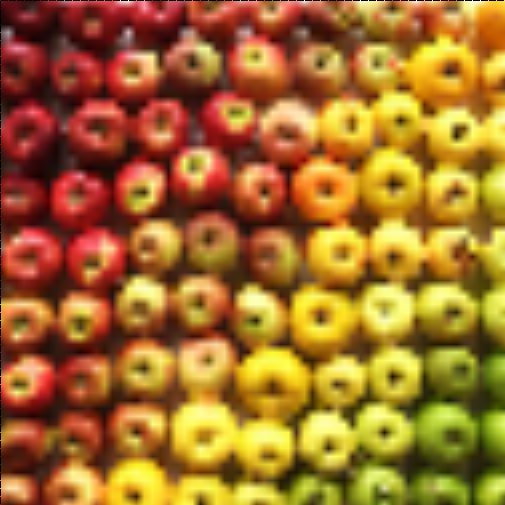
\includegraphics[width=4cm,height=4cm]{decompressed3.png}}
		\subfigure[6 descomprimida com h = 2 e k = 1 três vezes, err = 0.093727\label{surreal37}]{
		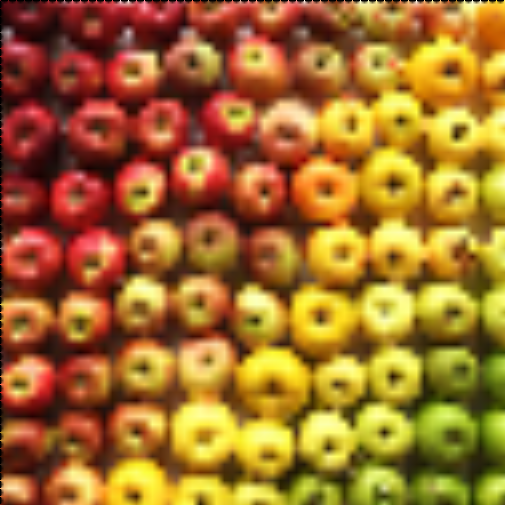
\includegraphics[width=4cm,height=4cm]{decompressed3b.png}}
		\subfigure[7 descomprimida com h = 5 e k = 5, err = 0.042874\label{surreal27}]{
		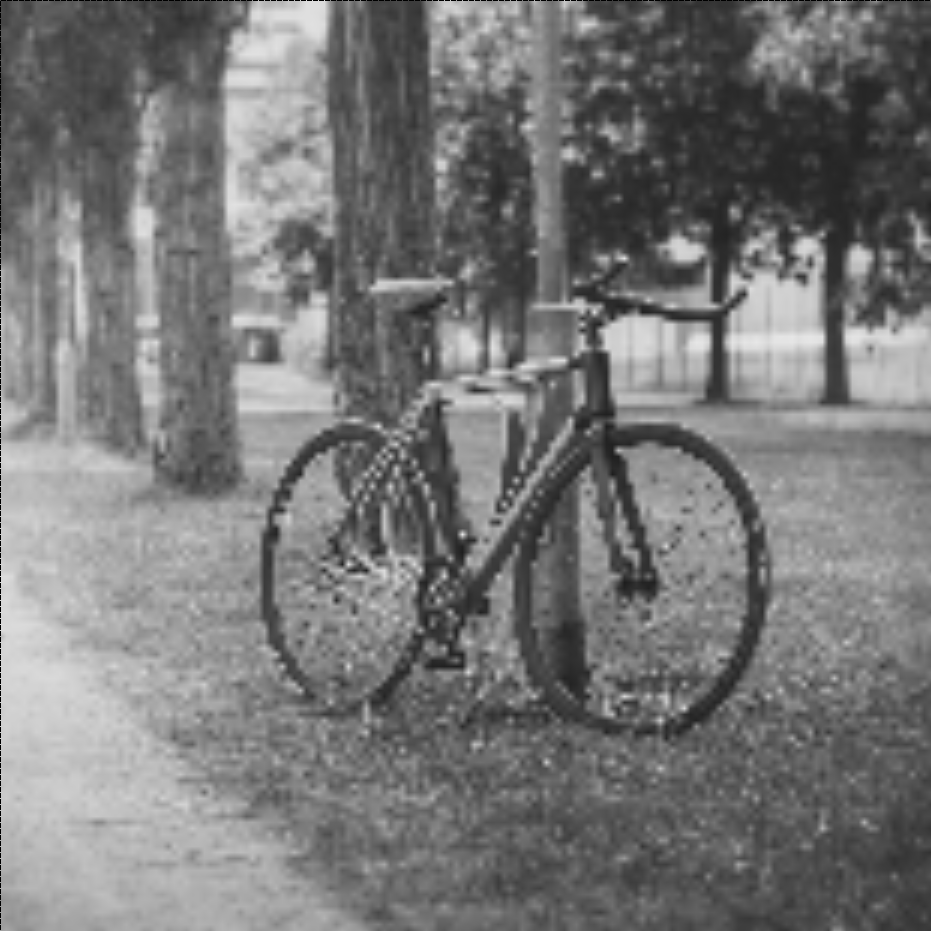
\includegraphics[width=4cm,height=4cm]{decompressed4.png}}
	\end{figure}
	
	\clearpage
		
	\subsection{Usando o método Bicúbico}

	Usando o método Bilinear, descomprimimos as imagens, e obtivemos as seguintes respostas para as perguntas do enunciado:
	
	\textbf{1.} Funciona bem para imagens preto e branco?\\
	\\
	
	\textbf{2.} Funciona bem para imagens coloridas?\\
	\\
	
	\textbf{3.} Como o valor de h muda a interpolação? \\
	\\
	
	\textbf{4.} Como se comporta o erro?\\
	\\
	
	\textbf{5.} Considerando uma imagem de tamanho $p^2$, comprimida com $k = 7$ e descomprimida com $k = 7$ e com $k = 1$ três vezes, quais são as conclusões?\\
	
	
	Seguem as descomprimidas:
	
	\begin{figure}[h]
		\subfigure[4 descomprimida com h = 4 e k = 3, err = 0.057363\label{surreal15}]{
		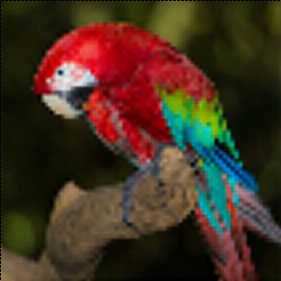
\includegraphics[width=5cm,height=5cm]{sbicdec1a.png}}
		\subfigure[4 descomprimida com h = 4 e k = 4, err = 0.067982 \label{surreal25}]{
		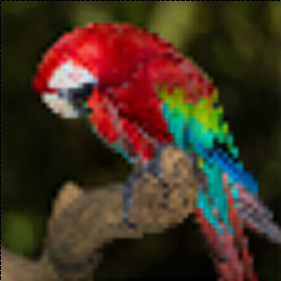
\includegraphics[width=5cm,height=5cm]{sbicdec1b.png}}
	\end{figure}
	
	\begin{figure}[h]
		\subfigure[5 descomprimida com h = 3 e k = 7, err = 0.033906\label{surreal16}]{
		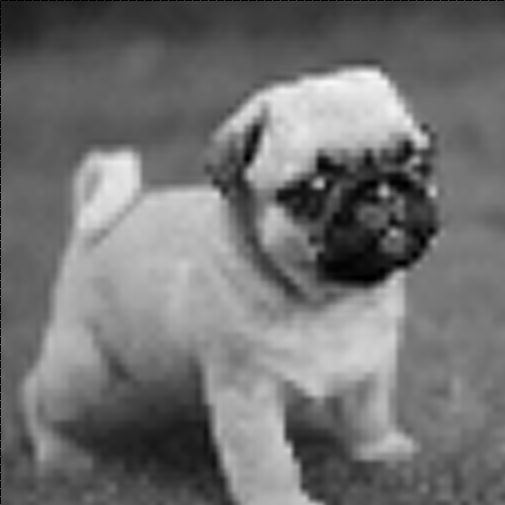
\includegraphics[width=5cm,height=5cm]{sbicdec2a.png}}
		\subfigure[5 descomprimida com h = 5 e k = 7, err = 0.033904\label{surreal26}]{
			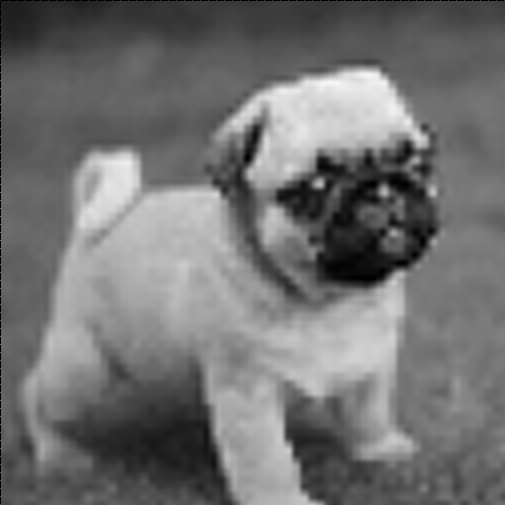
\includegraphics[width=5cm,height=5cm]{sbicdec2b.png}}
	\end{figure}
	
	\begin{figure}[h]
		\subfigure[6 descomprimida com h = 2 e k = 7, err = 0.079984\label{surreal17}]{
		
\includegraphics[width=4cm,height=4cm]{sbicdec3a.png}}
		\subfigure[6 descomprimida com h = 2 e k = 1 três vezes, err = 0.091454\label{surreal37}]{
		
\includegraphics[width=4cm,height=4cm]{sbicdec3b.png}}
		\subfigure[7 descomprimida com h = 5 e k = 5, err = 0.043302\label{surreal27}]{
		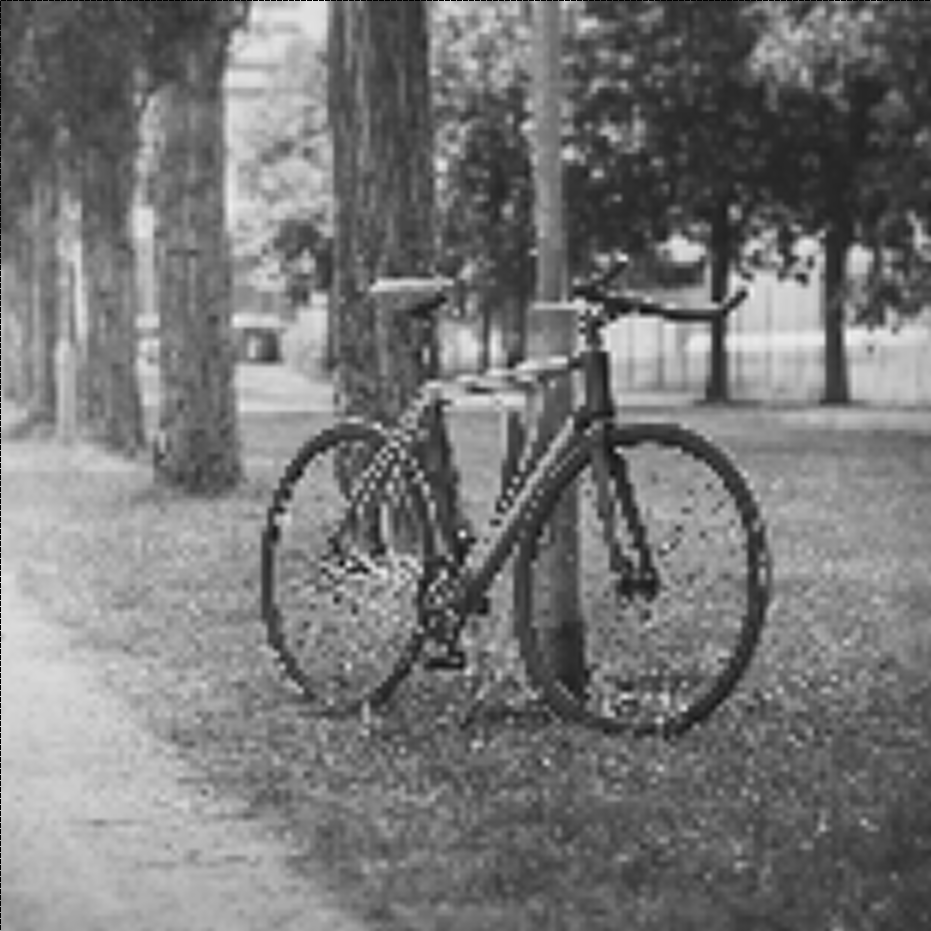
\includegraphics[width=4cm,height=4cm]{sbicdec4.png}}
	\end{figure}
	
\end{document}